he\chapter{System Maintenance}

\section{Environment}

\subsection{Software}

Below is the complete list of programs used when creating my system:

\begin{itemize}
	\item Python 3 (Programming Language the system was written in)
	\item IDLE (used to write the python scripts)
	\item PyQt 4 (Used to produce a user interface for the system)
    	\item SQLite 3 (Used to implement databases into the system)
	\item SQLiteInspector (Used to ensure data has been added to the database file correctly)
	\item Adobe Photoshop CS6 (Used for creating Graphics for the System)
	\item Microsoft Excel (Used to edit the CSV file)
	\item Notepad (Used to create the .txt file containing all of the counties in the UK.)
	\item Notepad + + (Used to write the HTML invoice)
	\item Google Chrome (Used to preview the HTML invoice and used to sign into a email client to view the emails sent to specific email addresses)
\end{itemize}

\pagebreak

\subsection{Usage Explanation}

\textbf{Python 3}
\begin{itemize}
	\item It is The Programming Language i am most familiar with.
	\item The Software is free to download
	\item Python is avaiable on all system platforms. Meaning the program can still be used if my client changes operating systems.
	\item There are a lot of pre installed modules, that i could use which means the user does not have to install many extra modules for my system to work.
	\item Python is an object orientated programming language
\end{itemize}
\vspace{5mm}

\textbf{Idle}
\begin{itemize}
	\item Comes Free with Python so reduces the amount of downloads and installations needed.
	\item IDLE is free and does not have any restrictions.
	\item Designed specifically for python.
\end{itemize}
\vspace{5mm}

\textbf{PyQt 4}
\begin{itemize}
	\item Designed specifically for implementing a Graphical User Interface in python (GUI)
	\item Has a huge range of available widgets that can be used.
	\item PyQt 4 is Available on all operating systems.
\end{itemize}
\vspace{5mm}


\textbf{SQLite 3}
\begin{itemize}
	\item SQLite 3 is included in the python download, which will reduce the amount of downloads and installations required.
	\item Can be used to create simple single user used databases.
\end{itemize}
\vspace{5mm}


\textbf{SQLiteInspector}
\begin{itemize}
	\item A Database inspect is not required for my client, however i used this software as it made observing data inputs into the database a lot easier.
	\item SQLiteInspector allowed me to test SQL Queries before implementing them into my system.
\end{itemize}
\vspace{5mm}

\pagebreak

\textbf{Adobe Photoshop CS6}
\begin{itemize}
	\item the photo editing software that i am most confident using and familiar with.
	\item Allowed to me to create high resolution images that could be saved as a .png
	\item images can be saved with transparencies to remove backgrounds from my images.
	\item Comes with a huge variety of tools which meant i did not have to install any addition tools to create the graphics for my system.
\end{itemize}
\vspace{5mm}


\textbf{Microsoft Excel}
\begin{itemize}
	\item A spreadsheet program in which i am familiar with, that allowed me to Edit the CSV file.
	\item The spreadsheet program in which i am most familiar with, did not allow me to open the CSV file because it was too large. Excel allowed me to open it with no problems.
	\item Allows you to save files as .csv files which allowed me to open and edit the CSV file.
	\item is a very widely used piece of software which means that lots of solutions and help is available, if i wasn't sure how to do something when using the software.
\end{itemize}
\vspace{5mm}


\textbf{Notepad}
\begin{itemize}
	\item Comes pre-installed on all Windows based computers.
	\item Is the text editor i am most familiar with and is extremely easy to use.
	\item Allows you to save your file as a huge variety of different file types, although i only needed to save it as a .txt file, which is very common.
	\item although it is only available on Windows systems, there are many of similar plain text editors that will do the same job that i needed, but can be used on other Operating systems.
\end{itemize}
\vspace{5mm}

\pagebreak

\textbf{Notepad ++}
\begin{itemize}
	\item Is available on Windows operating systems, in which both me and my client currently use.
	\item Allows documents to be exported as .html which is what i needed to use it for.
	\item it allowed me to preview my HTML invoice easily and quickly.
\end{itemize}
\vspace{5mm}


\textbf{Google Chrome}
\begin{itemize}
	\item Is available to download free, on all operating systems
	\item once chrome is installed, nothing else is required for it to function properly
	\item Is a very popular search engine, meaning many know how to use the software.
	\item Allowed me to see what my HTML invoice would look like.
	\item is supported by Notepad ++ which allowed me to preview my invoice quickly.
\end{itemize}
\vspace{5mm}


\subsection{Features Used}

\textbf{Python 3}
\begin{itemize}
	\item Is an object orientated programming language
	\item Has a wide selection of built in functions and modules in which i could use, for example the random and time module.
	\item Python 3 has some improved features compared to Python 2 such as not being able to compare between string and integers and floats.
\end{itemize}
\vspace{5mm}


\textbf{IDLE}
\begin{itemize}
	\item Has syntax highlighting which means code is easier to read.
	\item Has a `Run Module' feature which allows either the GUI to be previewed or you can view the CLI in the Python Shell.
	\item has useful keyboard short-cuts (i.e F5 to Run the Module) which increases the ease of use of the software and allows you to do things a lot faster.
	\item has to ability to find the line in which an error lies and highlights it for you. This allows debugging to be done much faster.
	\item has the ability to find certain keywords within your code, which is very useful when managing large python files. Being able to search for a specific function or variable allows you to find what you want a lot faster than searching manually.
	\item has a built in Debugger which helped me to debug problems in my system.
\end{itemize}
\vspace{5mm}

\textbf{PyQt 4}
\begin{itemize}
	\item Has a Huge selection of widgets available to use for the GUI.
	\item PyQt includes all the standard GUI features such as menus and toolbars.
	\item Supports SQLite 3
	\item Includes many Examples and Demos with the PyQt install that became very useful when trying to learn about PyQt and its features.
\end{itemize}
\vspace{5mm}

\textbf{SQLite 3}
\begin{itemize}
	\item I used SQLite 3 queries to Add, Edit and Remove data from the database.
	\item there is no configuration needed in SQLite 3.
	\item Creating a database is easy and SQLite 3 is widely used so examples and help can be found easily.
\end{itemize}
\vspace{5mm}

\textbf{SQLiteInspector}
\begin{itemize}
	\item Allows you to view all the tables within a database.
	\item Lets you test SQL Queries and displays the outcome of the query, without having to implement anything into the system.
	\item Allows you to view the entity descriptions to ensure referral integrity is enforced.
\end{itemize}
\vspace{5mm}

\textbf{Adobe Photoshop CS6}
\begin{itemize}
	\item Allows you to edit any image type.
	\item Allows you to keep transparency when saving the image as a .png
	\item Allows you to undo changes, which proved to be helpful when making unwanted changes.
	\item Many useful keyboard short-cuts, making creating graphics a lot faster process
\end{itemize}
\vspace{5mm}

\textbf{Microsoft Excel}
\begin{itemize}
	\item Has a search feature which allowed me to find the information i wanted easily, which was useful because the CSV file was extremely large.
	\item Microsoft Excel allows you to delete entire rows or entire columns, this is very useful when managing a large spreadsheet.
	\item Allows you to Find words and replace them with others. This proved useful when I wanted to capitalise the name of the towns within the CSV file.
	\item Allows you to export the file as a .csv
\end{itemize}
\vspace{5mm}

\textbf{Notepad}
\begin{itemize}
	\item Allows you to Copy and Paste plain Text into Notepad
	\item all the features of notepad are simple and easy to use.
\end{itemize}
\vspace{5mm}

\textbf{Notepad ++}
\begin{itemize}
	\item Syntax colouring which makes the HTML easier to read.
	\item Notepad ++ supports HTML syntax.
	\item keyboard short-cuts allowed me to create the HTML invoice a lot faster.
	\item Notepad ++ has been developed to maximise execution speed from minimal system resources.
\end{itemize}
\vspace{5mm}

\textbf{Google Chrome}
\begin{itemize}
	\item Is a lot faster than other search engines such as internet explorer, which meant previewing my invoice was fats and easy.
	\item The Tab feature allowed me to have two different invoices open at once and make comparative decisions between them which proved to be a useful feature.
	\item The bookmark feature allowed me to save my invoice as a bookmark and be able to view it whenever i am on google chrome. (Does not require Notepad ++ to be open).
\end{itemize}

\section{System Overview}

\subsection{Log In}

The Log in Screen prevents any unauthorized users from being able to access the system without logging in. When the user enters a user-name and password the system will then search the database for any users who match the credentials entered by the user.If the user-name and password the user enters match an account within the database, the user will be taken to the creating order interface as this will be the most used feature of the system. If the credentials do not match any of the accounts stored in the database, then the system will tell the user that their user-name or password is incorrect. If the user cannot remember either their user-name or password, they can click on the 'Forgot Username and Password button. Clicking this button will take the user to a screen where they must enter the email address associated to the account(This email address will have been added when the Employee was first created). The system will then search the database to see if the email address the user enters matches any of the employee accounts. If it does not, the user will be informed that the email address does not match any of the accounts, however, if it does, the User-name and Password of the Employee account will be sent to the email address also stored under the Employee account. If the user cannot access their email address to retrieve their Account details, the user will have to ask the administrator to change the email address associated to their account, to an email address that they can access.

\subsection{The Search Window}

The search window is a feautre of the system that allows the user to search for a product member or employee within the database. The user can access the search window by pressing CTRL+F on the keyboard simultaneously, or by clciking on the Search Window option under the Options meu in the menubar. In the search window the user has the ability to choose which table they would like to search, the product table, member table or the employee table. There is a search field that allows the user to enter any information and the table will dislpay any matching data. This is a very useful tool when wanting to find Products, Members or Employees.

\subsection{Create Order}

The Create Order interface allows an employee to create an order, from products currently being stored within the database. If the customer wants to purchase a product that is not currently being stored in the database, the employee will have to add the product to the database via the 'Add Product' interface before it can be added to an order. To add a product to the order, the user must find the product under the 'Find Product' table. To add the product to the order, the user can either click on the product then click then click the 'Add to Order' button or they can either double click on the product they want to add. If done succesfully the product should be added to the order and the subtotal, discount and total price should have changed. Once the Order is complete the user can then decide whether they want to print off the invoice, send it to an email address, or both. Once the Order has been created and the employee has decided whether to print or email the invoice, the employee can click the save invoice button which will send the invoice to the email specified or print off the invoice. If the customer is a member, the Employee can enter the customers MemberID and 10 percent of the price of the current order will be deducted.

\subsection{Adding Editing and Removing Products}

In order to be able to create an order, there must be products stored in the database. The Add Product interface allows the user to enter relevent information about the product along with an optional image of the product. The system validates the data the user enteres to ensure that the data is valid and is stored in a suitable format within the database. If the Employee wants to change the details about a product, for example the price, they must first find the productID of the product they want to edit or delete. This can be done easily using the search window which can be found under the Options Menu in the Menubar or by pressing CTRL+F when logged into an account. Once the user knows the ProductID of the product they want to edit, they can go to the Edit Product interface either by clicking on Edit Product under the Product Menu in the Menubar or by right clicking the product in the search window and clicking on the edit product option in the drop down menu. Likewise, if the user wants to delete a product, they can either go to the Delete Product option under the Product Menu in the Menubar or by right clicking on the product in the search window and selecting delete product from the dropdown menu.

\subsection{Managing the Stock of a Product}

If a product has been purchased in many orders, there may not but much stock left. If there are less the 5 of any specific product left in the shop, but many still left in storage, once a user logs on, the system displays a message telling them that the product needs to be restocked. If there are less than 5 in the shop and less than 5 in storage then the user is told that they should buy more stock. Once the user has bought more stock or has moved stock from storage to the shop, the must update this in the system. To do this, the employee must log into the system, then find the ProductID of the product they want to change the stock of. They enter the ProductID into the ProductID field in the Manage Stock interface. When the user clicks the find button, The Product Name, Image, Stock in Shop and Stock in storage will be displayed to the user. Here the user will be able to change the stock in each location. The suer will also be displayed a graph of the recent sales of that speciifc product, the data on this graph allows the system to be able to predict future sales of that product, this can aid the company in knowing how many of the product should be purchased when wanting to buy more stock.

\subsection{Adding Editing and Removing Members}
The company allows customers to join a membership scheme, which allows the customer to get 10 percent off all of their orders. To add a member to the system, the user can go to the 'Add Member' option under the Member Menu within the Menubar. Here, the employee must enter the details about the customer, such as their name, address, telephone number and email address. The employee can then save the member in the database. If the customer / member changes any of their information, they must inform the company so that they can change the information in their system. To edit a member, the employee must log into the system, then the employee must find the member by searching for any relevent information in the search window. To search for members in the search window the employee must choose the Member option from the Combobox, this should then display the Member table. Once the Employee has found the MemberID of the member, they can either right click on the member in the search window and click on the Edit Member from the drop down menu, or go to the 'Edit Member' option under the Member Menu in the Menubar. To delete a member from the system, the employee must find the Member in the search windwow, right click the Member and click on delete member, or enter their MemberID into the Remove a Member interface.

\subsection{Adding Editing and Removing Employees}
Realistically, the system will not be used by just one employee, therefore my system allows many employees to be able to use the system. When the system is first run, one Employee account is created which is the Admin account. The admin account will be able to access features of the system that a normal account will not. To add a new Employee account, the employee MUST sign in on the admin account, then the user can go to the 'Add Employee' option under the Employee Menu in the Menubar. Here the user can enter the name and email address of the new employee and then can save them to the database. Now the new account can be used to accessed the system. There is only one admin account, which cannot be removed from the system.
To edit or delete an employee account the user must log into the admin account. Then, the user must go to the search window and find the employee they want to delete, they can then right click on an employee and click either edit or delete employee.


\section{Code Structure}

%use as many subsections as necessary for the code sections

\subsection{Decision Pop Up Window.}
\begin{figure}[H]
\pythonfile[firstline=5,lastline=7]{./Maintenance/PopUpMenuClass.py}
\end{figure}

Above shows a section of code that creates a Decison Pop up window where the user will be displayed a message and will have decision to make i.e (Yes or No, Ok or Cancel)
Obviously, in my system i will need to have more than one Decision pop up window, therefore i decided to make the Pop up window a class. This means many different instances of the pop up window can be made without having to repeat code. The above snippet shows the constructor of the class and shows the information that must be passed into each instance. Passing This data into the constructor allows different pop up windows to be made from the same class. The three things that get passed into the constructor, are the message that is displayed on the Pop up Window and the two buttons that are on the Pop Up Window(i.e Ok, Cancel, Yes, No.)

\subsection{Deleting Product Function}
\begin{figure}[H]
\pythonfile[firstline=33,lastline=39]{./Maintenance/AddingremovingData.py}
\end{figure}
 Above shows the function that is used to remove Products from the database. It is obvious that the user may want to delete many products from the system therefore, i decided to create a Function that allows the user to delete Products. I decided to make this a function as it will allow the user to be able to repeat the process of deleting a product over and over. The information that is passed into the function is the ProductID of the Product to delete, this allows the user to be able to use one function to be able to remove an infinate amount of products from the system wihtout having to repeat any code.

\subsection{Table used for the Search Window}
\begin{figure}[H]
\pythonfile[firstline=192, lastline=222]{./Maintenance/FindingPopUpClass.py}
\end{figure}

The above snippet shows the method used to change the model of the table. I decided to use a QModel and a QTableView in order to display the data from the database because it allowed me to switch between tables in the database. In The search window, the user can either search for a product memeber or employee. To switch between the tables, the user tells the system what they want to search for by selecting one of the options from a combobox. The model of the QTableView is then changed depending on the currently selected item in the ComboBox. This allows me to switch between different Models and keep the same table. If i did not use models, i would have to create a unique table for product, memebr and employee achange which one is viewed. Using models and switching between them requires a lot less code and means i do not have to repeat any code.

\subsection{Adding and Removing Data}
\begin{figure}[H]
\pythonfile[firstline=324,lastline=365]{./Maintenance/AddingRemovingData.py}
\end{figure}

The Above shows a small section of my AddingRemovingData file. This file contains all of the SQL statements that are used in the system. The reason that i have put all the SQl statements into one file is that it makes it much easier to find specific SQL statements when i need to because i know that they're all in the same file. If i put the SQL statements in the files where they are needed, it would make it harder to find the SQL statements i am looking for.

\subsection{Organisation of Classes.}
\begin{figure}[H]
    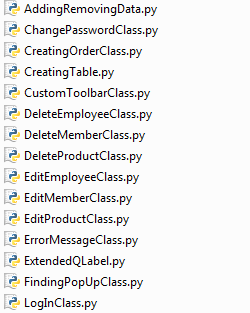
\includegraphics[width=\textwidth]{./FilesExample.png}
\end{figure}

The Above does not show the structure of my code as such, however it shows that i have seperated each class into its own individual file. I have split each class into its own file as this made it a lot easier when trying to debug problems with my code. For example if i know there was something wrong with Editing a Product, i would instantly know that i would have to look at EditProductClass.py . This made finding problems in my code very easy compared to if i had grouped many classes into one file. It also helped to shorten the length of each file, which means the contents of each file can be organised a lot easier.

\subsection{Table used for the Search Window}
\begin{figure}[H]
\pythonfile[firstline=66, lastline=71]{./Maintenance/AddingMemberClass.py}
\end{figure}

The above code shows how the County ComboBox is populated. During the Implementation stage i know it would be very long and tedious, hard coding each and every county in the UK into the ComboBox. Therefore, i created a text file containing all the counties, each separated with a comma. From here i could use python to extract each county from the text file and add it to a list. Line 70 from the code above shows a FOR loop, which places each item into the ComboBox. Using a For loop allowed me to reduce the amount of code compared down to 2 lines, compared to hard coding each county into the Combobox. 

\subsection{Emailing Functionality}
\begin{figure}[H]
\pythonfile[firstline=650, lastline=674]{./Maintenance/Main.py}
\end{figure}

The above code shows the exception handling when trying to send an email. I have used exception handling for common errors that occurred during the implementation stage when trying to send emails. The two common errors i had when trying to send emails was the credentials used to send the email were not valid, and not being connected to the Internet. If either of these problems occur, the user is now displayed with an appropriate message telling them why the email could not be sent. I also included a third except statement that will cover any other problems that may occur when sending an email, however there is no way to specify to the user what the problem is. Putting these except statements in greatly reduced the chance of my system to break when being used.

\subsection{Validation Function}
\begin{figure}[H]
\pythonfile[firstline=256, lastline=260]{./Maintenance/AddingMemberClass.py}
\end{figure}

The function above shows how the Members Postcode is validated. In order for the postcode to be valid, the text entered by the user must match the regular expression for the postcode. Using a regular expressions allows many different postcodes to be valid, without having to specify exactly which postcodes are valid. For example saying that the exact postcode 'CB7 5LQ' is avalid as apposed to saying : "if the postcode starts with 2 letters followed by a number then it is valid. This section of code is a Function because it reduces the repetition of code and gets called every single time the text in the postcode field is changed. 

\pagebreak

\section{Variable Listing}

You can find my data dictionary on Page 104 

    \begin{longtable}{|p{1.5cm}|p{4.5cm}|p{2cm}|p{2cm}|}
        \hline
        \textbf{Variable Name} & \textbf{Purpose} & \textbf{Section} & \textbf{Line Numbers}\\ \hline
	self.title & The Text that is displayed at the top of each Interface & & \\ \hline
	encrypted-password & stores the password after it has been encrypted & & \\ \hline
	decrypted-password & stores the password after it has been retrieved from the system and decrypted. & & \\ \hline
	self.valid & is a boolean variable to say whether a method returns true or false. & & \\ \hline
	subject & used to store the Subejct of the email that is sent to the customer / employee & & \\ \hline
	send-from & used to store the email address the email is sent from & & \\ \hline
	self.code & The random 4 digit code that is generated when an Employee wants to reset their password. & & \\ \hline
	employee-info & stores the information about an employee so that it can be used in an email. I.e the password reset email says: Hello ... where ... is the name of the employee. & & \\ \hline
	self.spacer & used to add spacing between widgets & & \\ \hline
	self.vertical-spacer& used to add vertical spacing between widgets & & \\ \hline
	first-name & used to store the first name entered by the user & & \\ \hline
	last-name & used to store the last name entered by the user & & \\ \hline
	full-name-list & Used to store the First letter of the First Name, The last name and the EmployeeID. & & \\ \hline
	self. pattern & used as a variable for the regular expressions used in the validation & & \\ \hline
	self. postcode-input & used to store a postcode to check if the postcode is i the CSV file. & & \\ \hline
	self. county-list & A list used to  store all the counties in the UK & & \\ \hline
	self. scaled-image & a a variable used to store a QPixmap that has been scaled to a specific width and height & & \\ \hline
	path & used to store the path of the Product Image selected by the user & & \\ \hline
	rows- in-table & used to store the amount of rows currently in a table & & \\ \hline
	self. file-name & used to store the New ProductID of the image going to be stored. & & \\ \hline
	self. temp & used to store a temporary value & & \\ \hline
	self. category-string & used to turn the combobox selection by the user into string. For example if the user selected Dog and Food from the combo-boxes, self. category-string would store the string 'Dog Food'.& & \\ \hline
	Product & used to store a list of all the Product information & & \\ \hline
	order -info & used to store a string of all the information related to an order & & \\ \hline
	data & variable used to turn individual variables into a tuple. & & \\ \hline
	date -stored & variable used to store the last sales date from the settings table & & \\ \hline
	date & used to  todays current date & & \\ \hline
	date -time & stores the current time in hours and minutes & & \\ \hline
	invoice -date & stores the date the invoice was created & & \\ \hline
	new -date & stores the todays date + 7 days (1 week) & & \\ \hline
	greatest -employee-id & stores the highest EmployeeID in the database & & \\ \hline
	new -employee-id & adds 1 to the highest EmployeeId to create a new EmployeeID & & \\ \hline
	move -list & stores the ProductID of all the products with a stock in Location 1 less than 5 & & \\ \hline
	restock -list & stores the ProductID of all the products with a stock in Location 1 and Location 2 less than 5. & & \\ \hline
	total -stock & adds the stock in Location 1 to the stock in location 2 and stores this value. & & \\ \hline
	self. subtotal-price & adds the prices of all the Products currently in the order and stores this value.& & \\ \hline
	self. total-price & stores the value from (self.subtotal-price - self.discount) & & \\ \hline
	self. money-off & calculates (self .total-stock * 0.1) and stores the value & & \\ \hline
	invoice -history & is an array that stores the date and time the invoice was made and the date and time the invoice was sent & & \\ \hline
	html & used to store the HTML invoice that is either printer or emailed to a customer& & \\ \hline
	\end{longtable}
	
	
	
	


\section{System Evidence}

\subsection{User Interface}

\begin{figure}[H]
    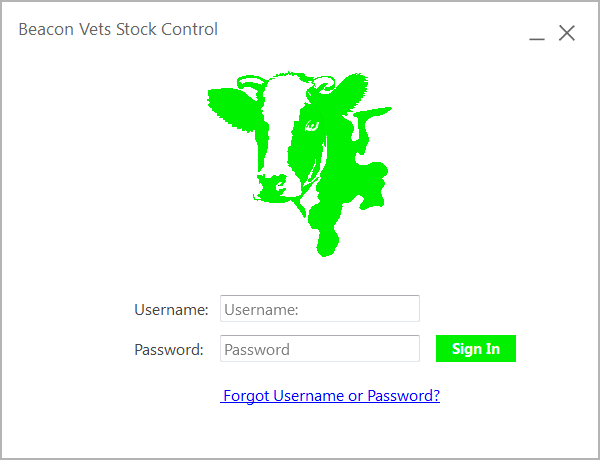
\includegraphics[width=\textwidth]{./interface1.png}
    \caption{Logo In Interface} \label{fig:log-in-interface}
\end{figure}

Figure \ref{fig:log-in-interface} is my log in interface. The figure below shows the Widgets and Layouts used to create the log in interface. 

\begin{figure}[H]
    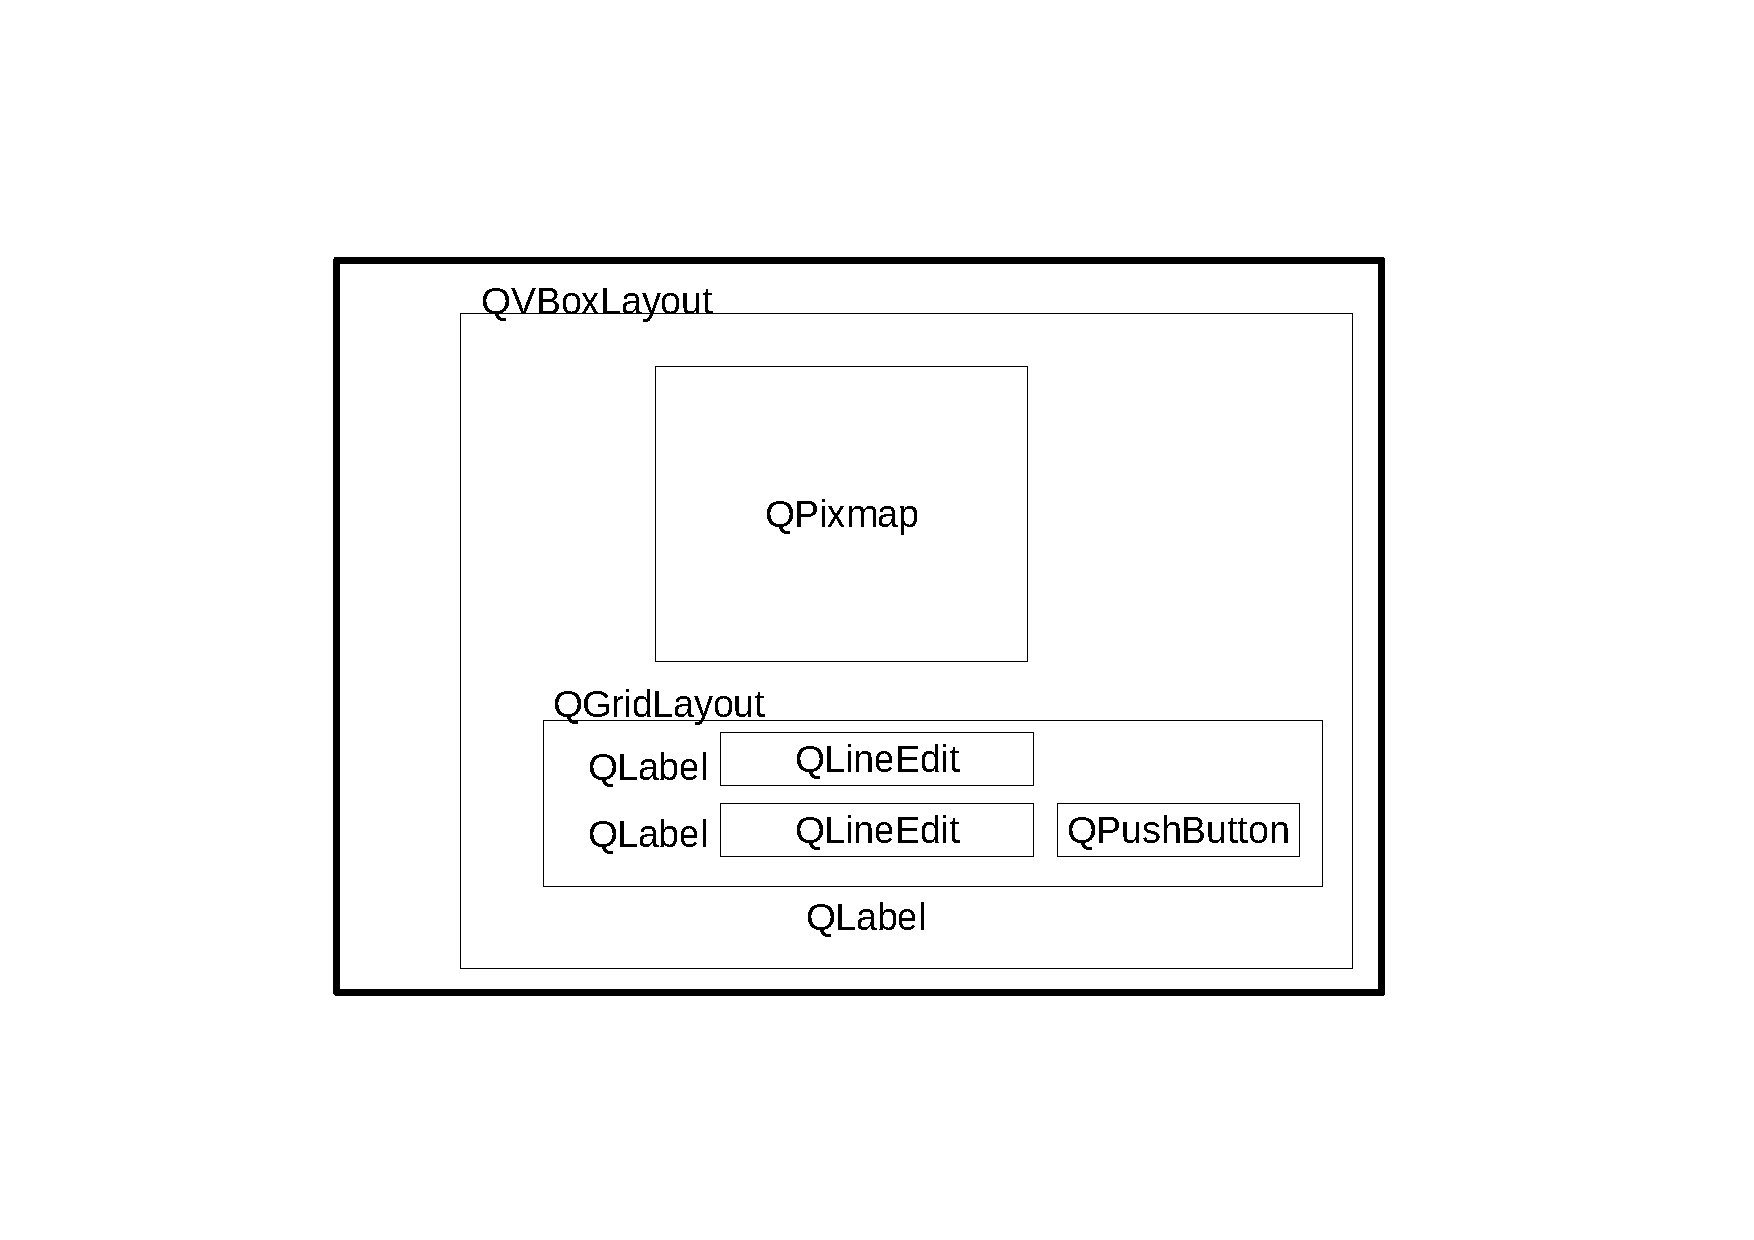
\includegraphics[width=\textwidth]{./structure-log-in.pdf}
    \caption{Structure of the Log In Interface} \label{fig:log-in-structure}
\end{figure}

The Log in Interface is built up from many widgets. The QPixmap is the logo of the company, The QLabels within the Grid layout tell the user what to enter into the QLineEdits. The QPushButton is the button in whihc the user presses once they have entered their log in details. If The user forgets their account details they can click on the Forgot Password Label which is the QLabel underneath the QGridLayout.

\begin{figure}[H]
    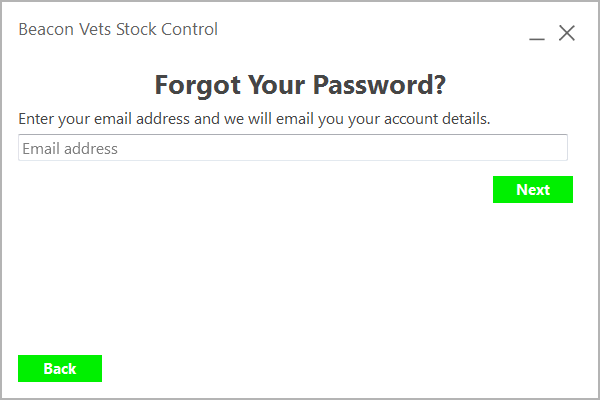
\includegraphics[width=\textwidth]{./interface2.png}
    \caption{Forgot Password Interface} \label{fig:forgot-password-interface}
\end{figure}

The forgot password interface has a QLabel with a unique style sheet that makes the text size larger and makes the text bold. This QLabel is the text that says: `Forgot Your Password.' This same style sheet has been used for all the other titles on each interface to tell the user what interface they are currently on. The forgot password interface then has a QLabel telling the user what to enter into QLineEdit. There is a QLineEdit in which the user can enter their email address and a QPushButton in which the user can click when they have entered their password. When the button has been clicked the database is searched for the email address the user entered. There is also a QPushButton in the Bottom left hand corner of the interface which the user can click to go back to the log in interface. This QPushButton was positioned in the bottom left corner using spacers which are just QWidgets that cannot be seen by the user.


\begin{figure}[H]
    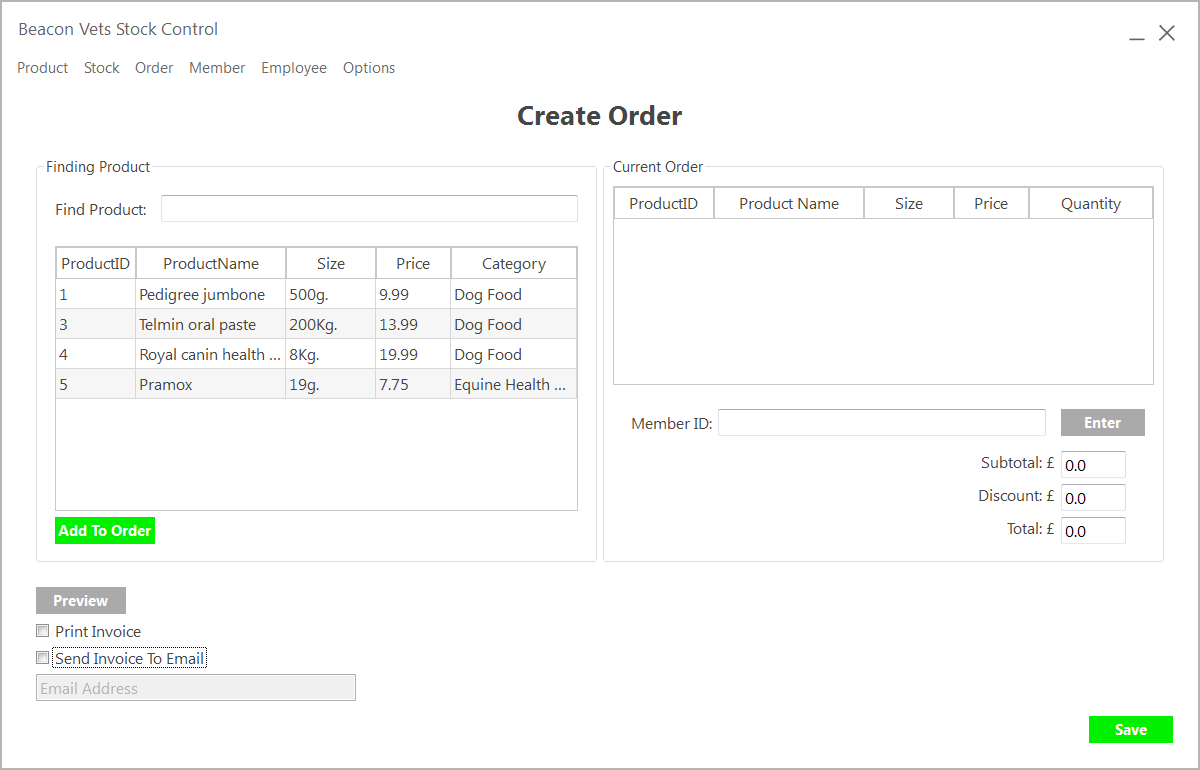
\includegraphics[width=\textwidth]{./interface3.png}
    \caption{Creating Order Interface} \label{fig:creating-order-interface}
\end{figure}

The create order interface was the most complex interface to design as it had to include many more widgets, compared to the other interfaces. below i have provided a diagram of all the widgets and layouts used to create the create order interface.

\begin{figure}[H]
    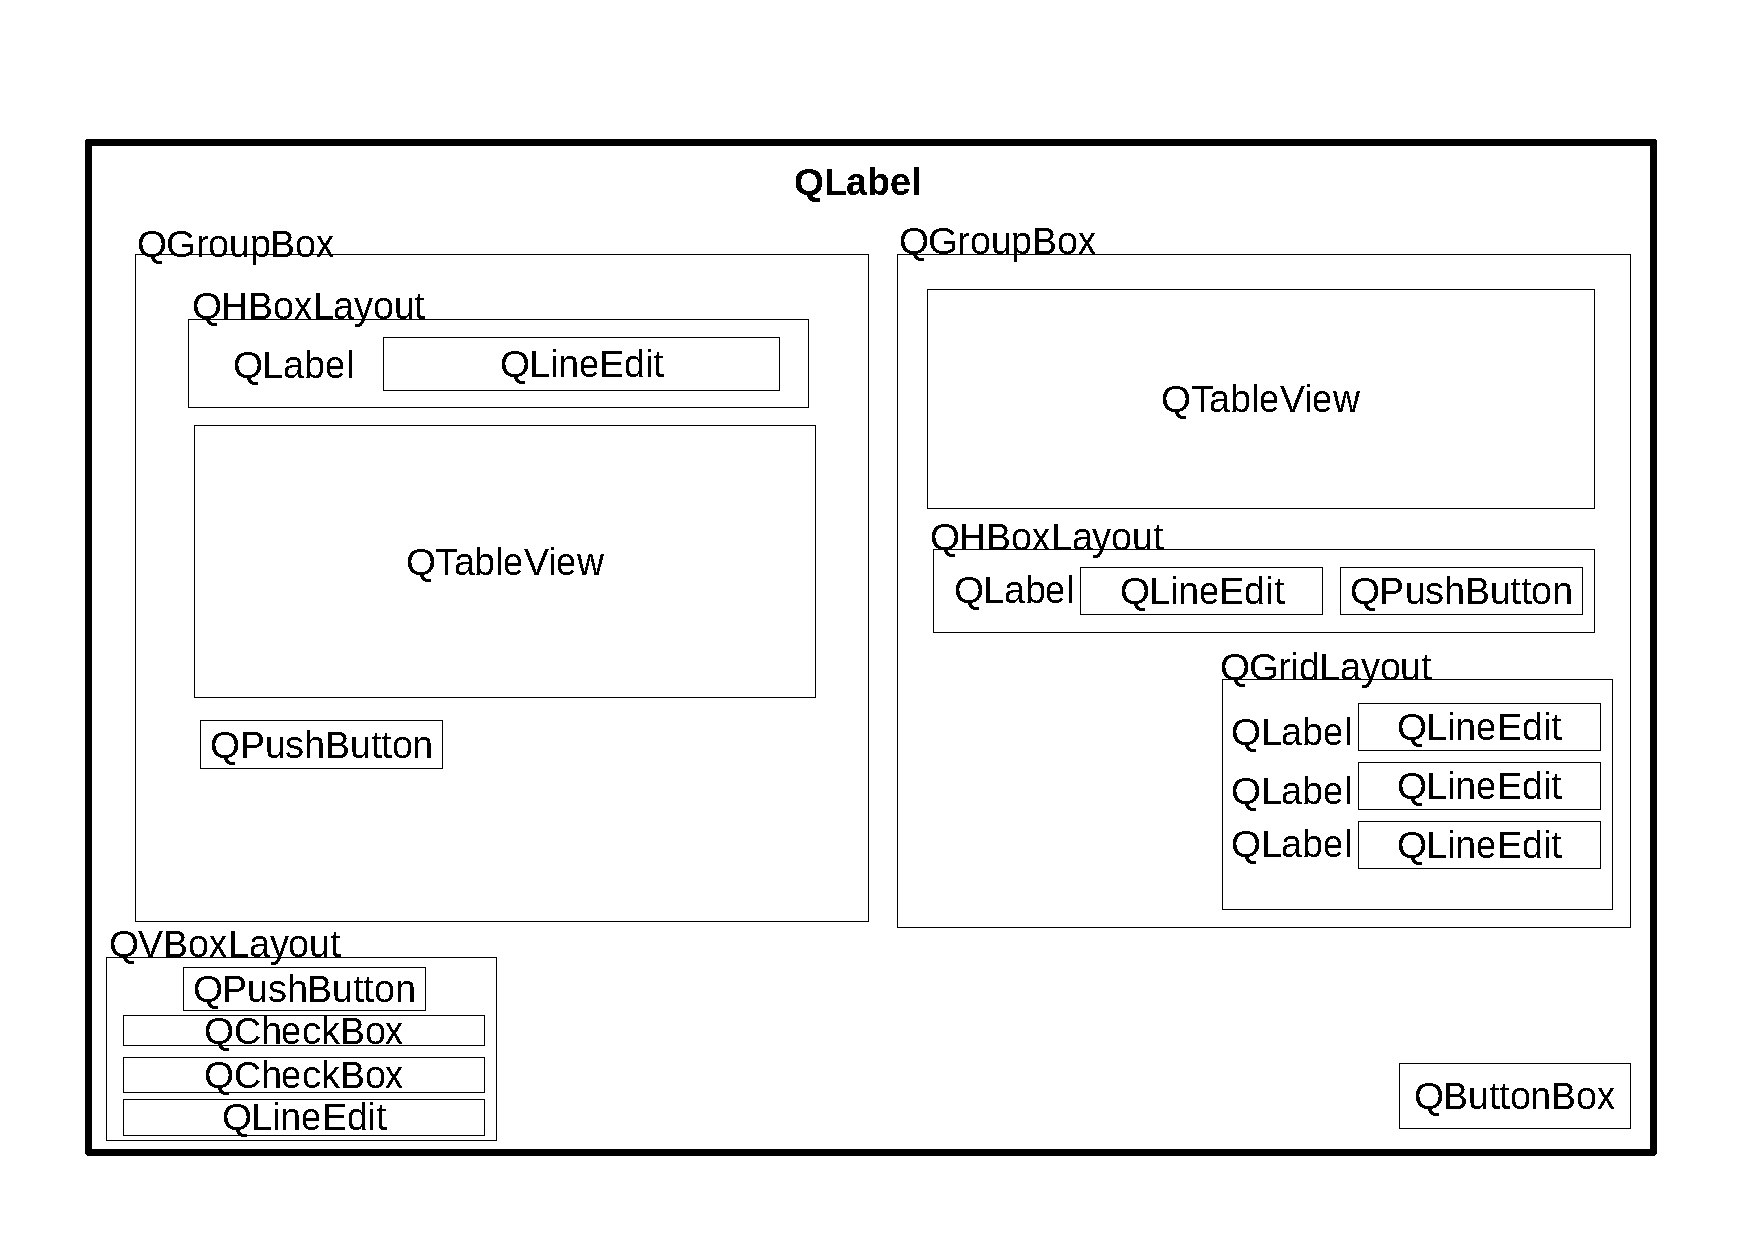
\includegraphics[width=\textwidth]{./structure-order.pdf}
    \caption{Structure of the Order Interface} \label{fig:structure-order}
\end{figure}

The QLabel in bold at the top of the page is the title of the page. This QLabel has a unique stylesheet as explained before, which gives the text are larger font and is in bold. The QGroupBox on the left is for the user to find a product. the QTableView in this QGroupBox displays the Product Table from the database. If the user enters any any characters into the QLineEdit within this group box, the system searches the Product Table for whatever the user entered and will display it in the table. This allows the user to search for specific products. The QPushButton in the QGroupBox will allow the user to add a specific product to the order if they have selected one in the table. Alternatively, the user can double click on a product in the table. The QGroupBox on the right is for the current order. the QTableView displays all the products that are currently in the order. When a user adds an item from the Product Table to the order, that product should be displayed in the current order table. Members get a 10 percent discount, therefore, there is a field that allows the user to enter a member id and the system will deduct 10 percent of the total price from the subtotal. The QLabels and QLineEdits in the QGridLayout display to the user; the subtotal of the order, the amount of money the customer gets off due to discount and the final price of the order after discounts. At the bottom of the page is where the user can decide how they want to output the invoice. The QPushButton allows the user to preview the invoice to ensure all the products have been added successfully. The two QCheckBoxes allow the user to either print the invoice, send it to an email or both. The QLineEdit in this QVBoxLayout allows the user to enter the email address to send the email to. The QButtonBox contains the save button where the user can save the Order to the database and they invoice can be printed or emailed.

\begin{figure}[H]
    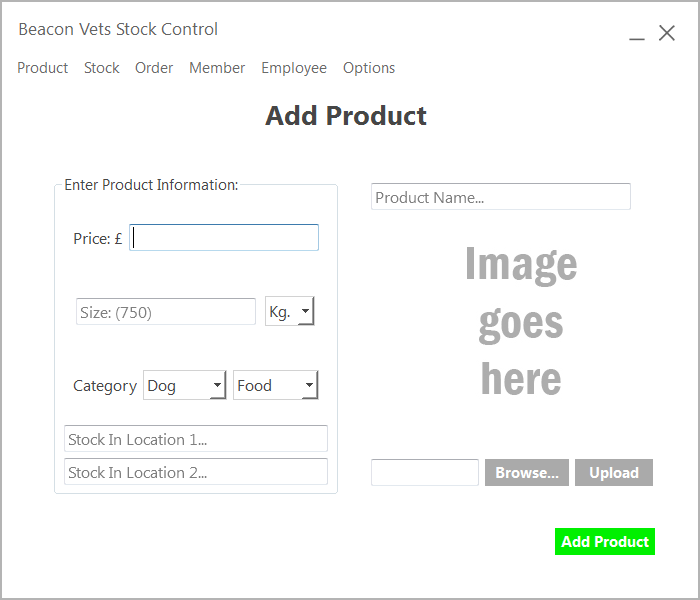
\includegraphics[width=\textwidth]{./interface4.png}
    \caption{Add Product Interface} \label{fig:add-product-interface}
\end{figure}

The Add Product interface contains 6 QLineEdits. 5 of the QLineEdits are for the Employee to enter the product information and one is for displaying the image path to the user. The QLineEdit for displaying the image path has been set to Read Only so that the user cannot edit the path. The QLineEdits for the data inputs allow the user to enter letters, numbers and special characters. After creating my system, i feel it would have been more sensible to use QSpinBoxes for the stock inputs as these only allow integers to be entered into the field. I have used some QLabels to tell the user what to enter into the field, however this is also done by the place holder text within the QLineEdits. I have used two QPushButtons, one allows the user to search for the image, the other updates the QPixmap so that it displays the image selected to the user. The QPushButton in the bottom right corner allows the user to save the product. Once they have entered data into all the fields they can click this button to add the product to the database.


\begin{figure}[H]
    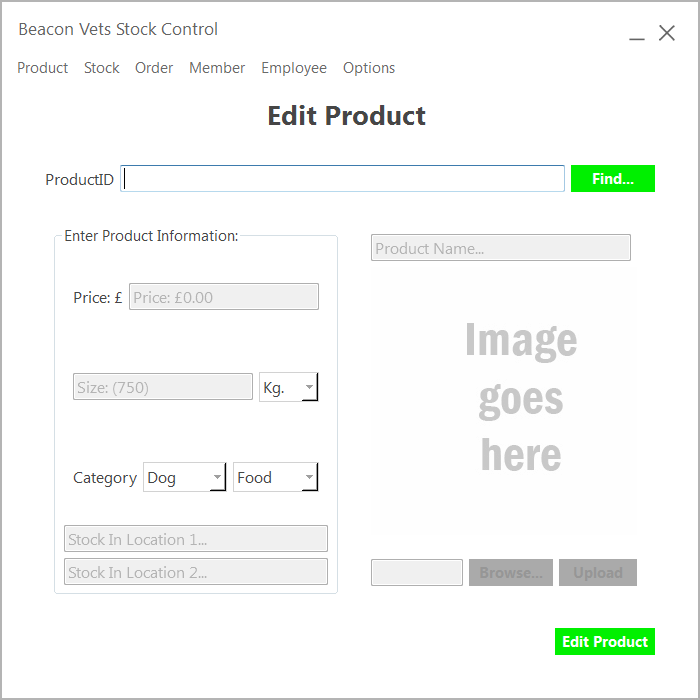
\includegraphics[width=\textwidth]{./interface5.png}
    \caption{Edit Product Interface} \label{fig:edit-product-interface}
\end{figure}

The Edit product interface is similar to the add product interface however there is an additional widget between the title and the main widget. The additional widget is a QLabel, QLineEdit and QPushButton in a QHBoxLayout. The QLabel tells the user what data needs to be entered into the QLineEdit (ProductID), and the QPushButton searches the database for the data the user enters. Until a Product has successfully been found, all the widgets inside the main widget have been disabled which means the user cannot enter data into them. The Edit Product push button has also been disabled.
\begin{figure}[H]
    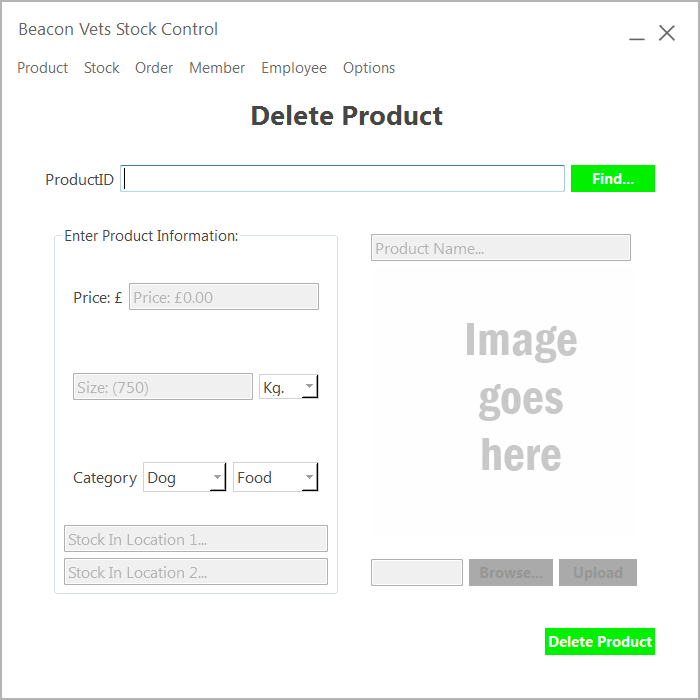
\includegraphics[width=\textwidth]{./interface6.png}
    \caption{Removing Product Interface} \label{fig:removing-product-interface}
\end{figure}

Visually, the Edit and Delete Product interfaces look extremely similar. however there are some slight differences in their functionality. Once the user has found a product, in the Delete Product interface, the data fields are set to read only. This means the user cannot edit the data in the data fields. Also, when the user finds a product in the delete member field, no validation takes place because no data is being changed and the data should have been valid when it was input originally. When the user clicks the delete product push button, the system searches for the product id and removes it from the database.

\begin{figure}[H]
    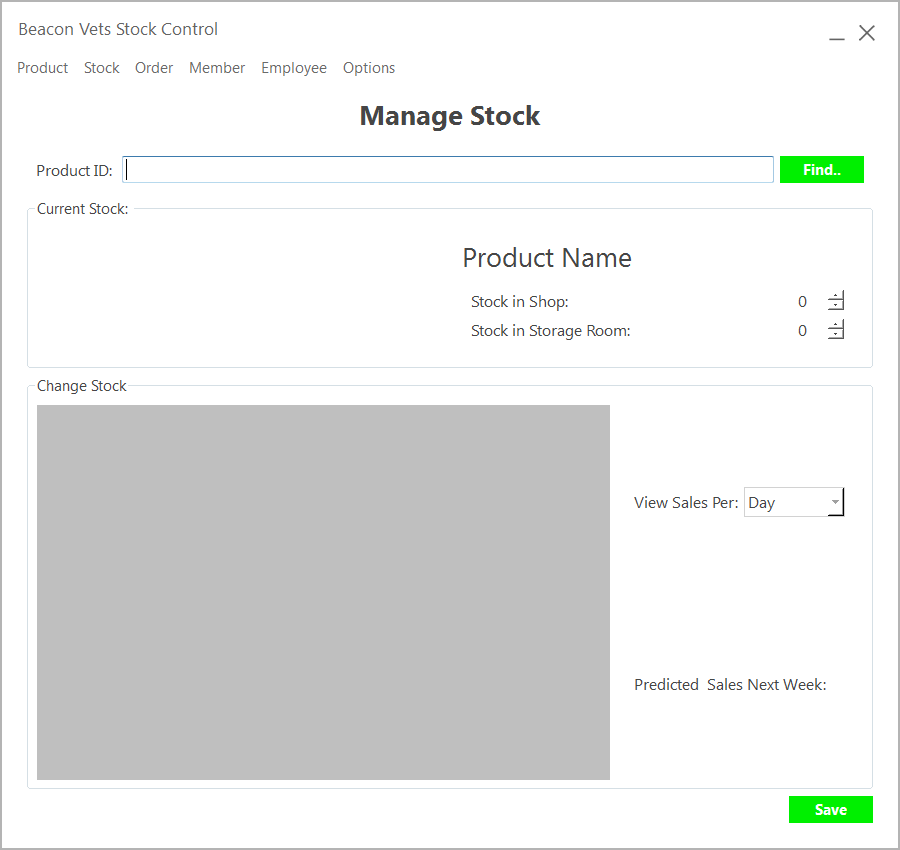
\includegraphics[width=\textwidth]{./interface7.png}
    \caption{Manage Stock Interface} \label{fig:stock-interface}
\end{figure}

The Manage stock interface contains three widgets inside a QVBoxLayout. There is the Widget in which the user enters the ProductID of the Product they want to edit the stock of, The Current Stock groupbox which shows the current stock of the product in the database, along with displaying the product name and product image to ensure the user is editing the stock of the correct product. The Other GroupBox shows the sales of that product over a period of time. The graph displays the amount of sales made on a specific date. Inside this GroupBox there is a QComboBox that allows the user to change the graph to show either the sales made each day, or sales made each week. The graph also works out the predicted sales for the following week, which is output to the user in a QLineEdit that is set to Read Only. The save button in the QButtonBox allows the user to save the new stock if they changed it.

\begin{figure}[H]
    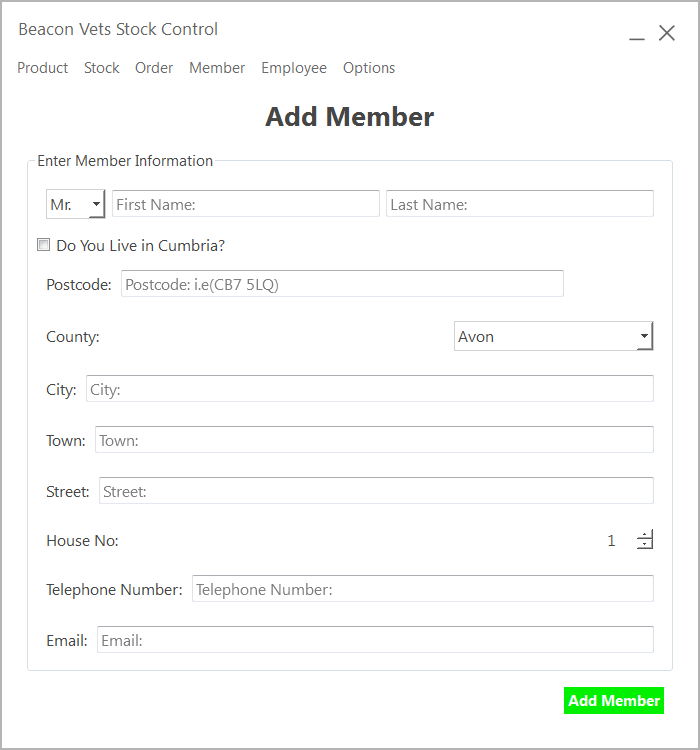
\includegraphics[width=\textwidth]{./interface8.png}
    \caption{Add Member Interface} \label{fig:add-member-instance}
\end{figure}

The Add Member interface has many QLineEdits, in which the user enters data about the Member. A QComboBox has been used for the Title (i.e Mr. or Mrs), and the county. The House Number field is a QSpinBox as the only allows the user to enter an integer. The state of the QCheckBox depends on whether a QPushButton is displayed. If the user does live in Cumbria, the user can click the checkbox which will cause a push button to appear. clicking this push button will search a CSV file containing all the postcodes and towns of all the postcodes in Cumbria. If the postcode is in the database the county and town field will be filled out automatically. This is to decrease the amount of time the user must spend to physically type information into the system.


\begin{figure}[H]
    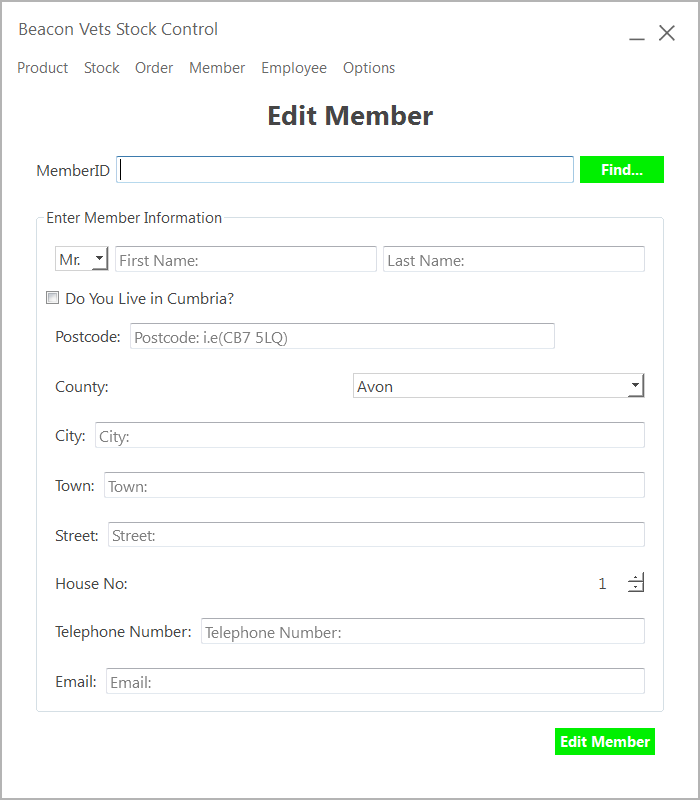
\includegraphics[width=\textwidth]{./interface9.png}
    \caption{Edit Member Interface} \label{fig:edit-member-instance}
\end{figure}

The Edit Member interface is very similar to the add member interface however it has a widget between the Title of the interface and the main widget. The new widget contains a QLabel that tells the user what to enter into the QLineEdit, a QLineEdit where the user enters the Member ID and a QPushButton, that when pressed, searches the database for a MemberID that matches the MemberID entered by the user. 

\begin{figure}[H]
    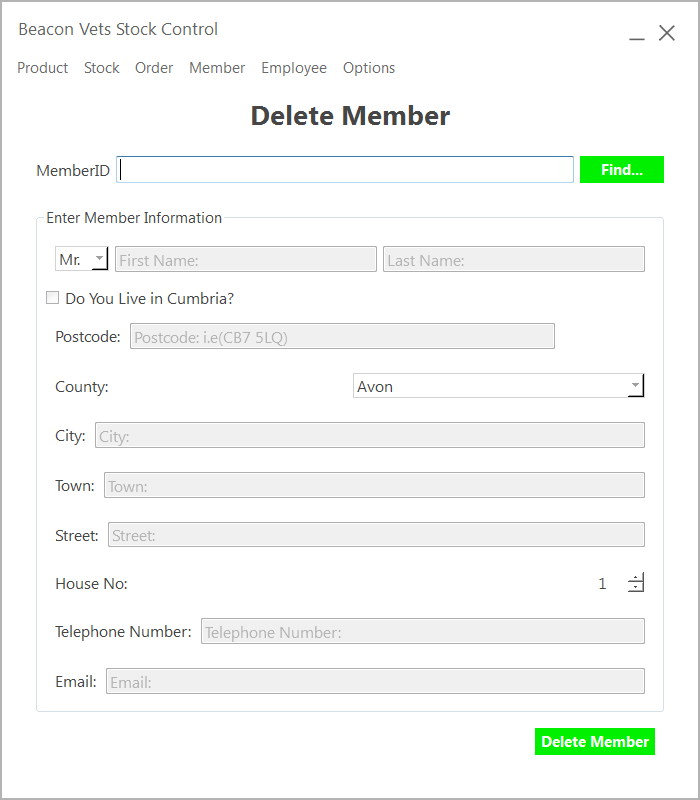
\includegraphics[width=\textwidth]{./interface10.png}
    \caption{Removing Member Interface} \label{fig:removing-member-interface}
\end{figure}

The Delete Member interface is visually identical to the Edit Member interface, other than the text on the QPushButton in the bottom right hand corner of the interface. When the Delete Member button is clicked, the system searches the database for the MemberId entered by the user and is removed from the system.

\begin{figure}[H]
    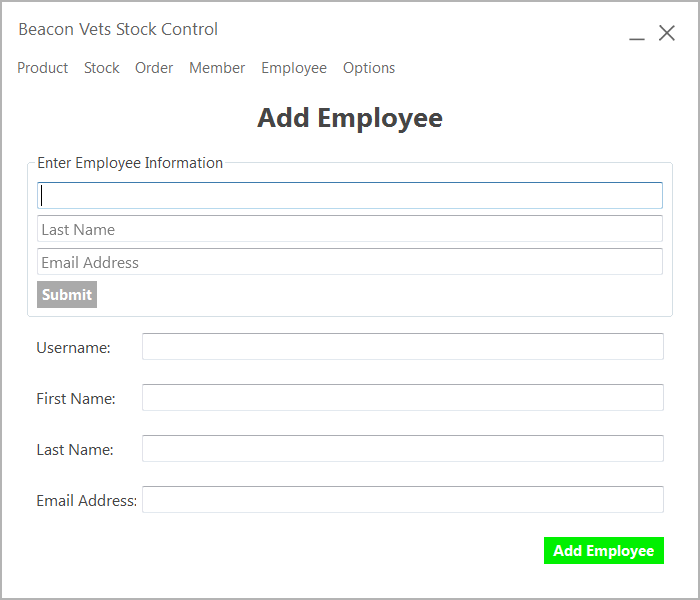
\includegraphics[width=\textwidth]{./interface11.png}
    \caption{Add Employee Interface} \label{fig:adding-employee-interface}
\end{figure}


\begin{figure}[H]
    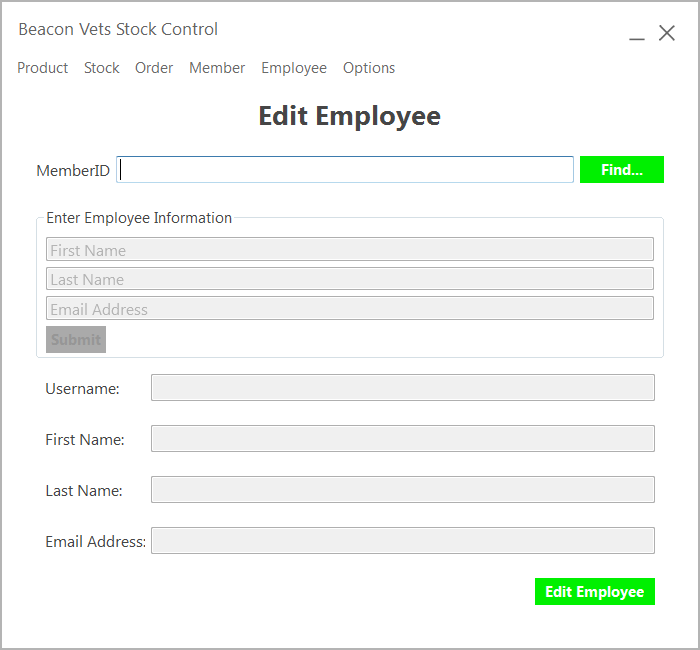
\includegraphics[width=\textwidth]{./interface12.png}
    \caption{Edit Employee Interface} \label{fig:edit-employee-interface}
\end{figure}

\begin{figure}[H]
    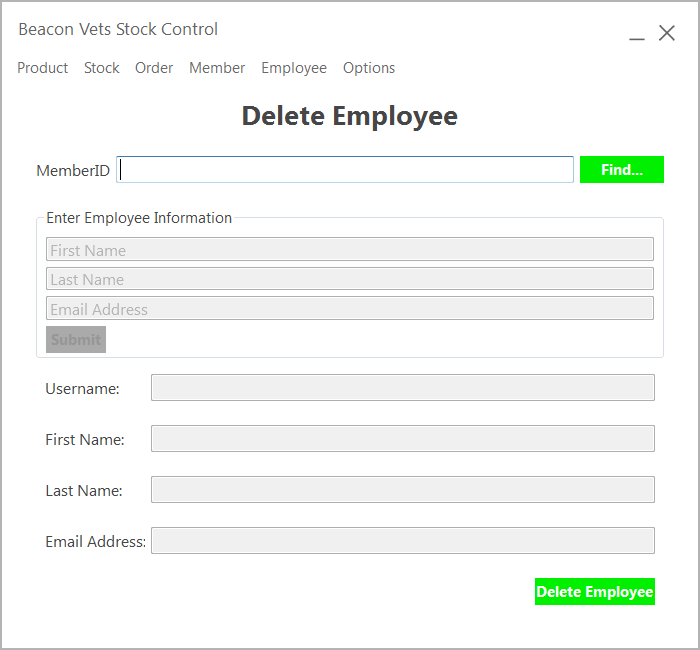
\includegraphics[width=\textwidth]{./interface13.png}
    \caption{Remove Employee Interface} \label{fig:removing-employee-interface}
\end{figure}

\begin{figure}[H]
    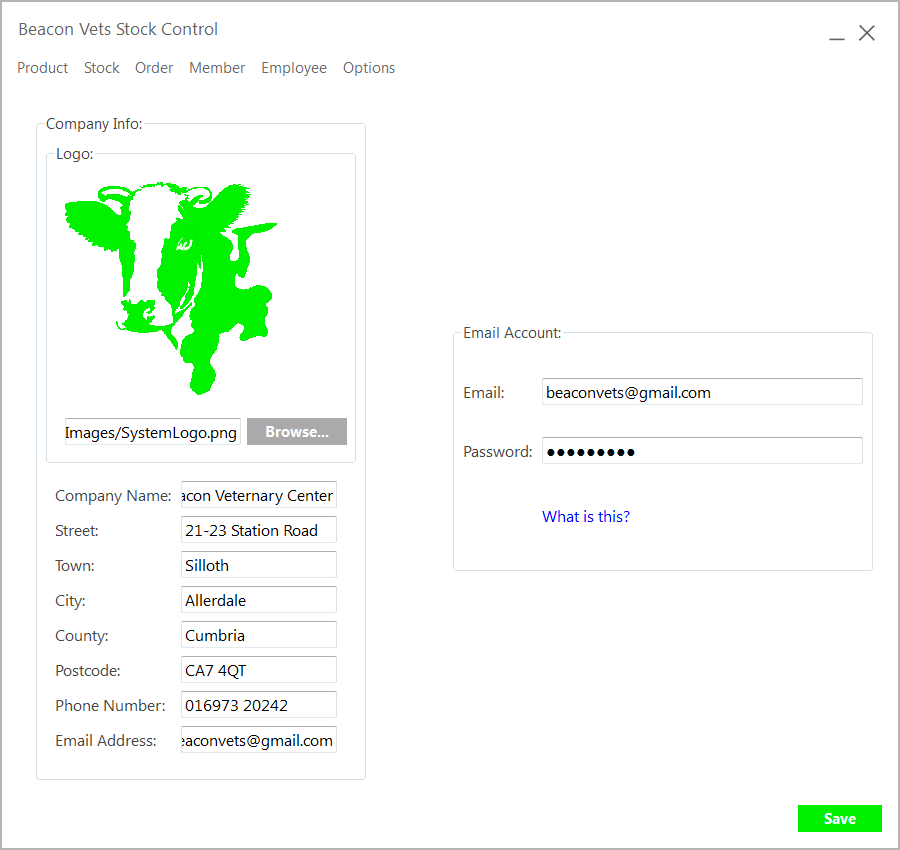
\includegraphics[width=\textwidth]{./interface14.png}
    \caption{Preferences Interface} \label{fig:preferences-interface}
\end{figure}

\begin{figure}[H]
    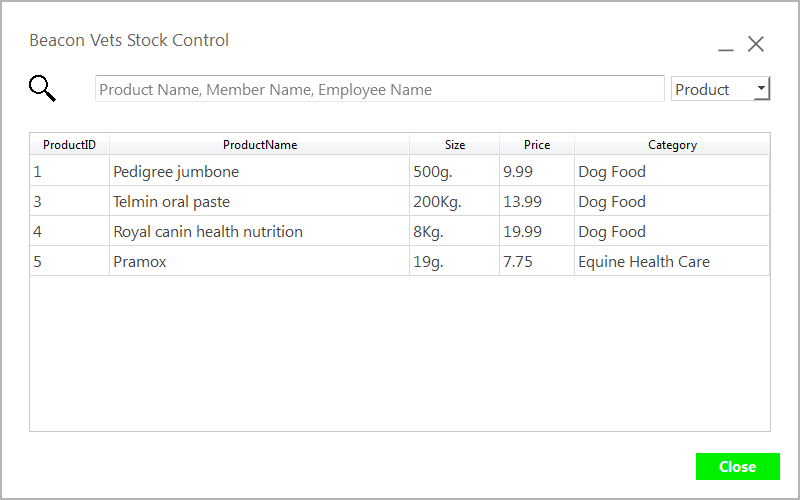
\includegraphics[width=\textwidth]{./interface15.png}
    \caption{Search Interface} \label{fig:search-interface}
\end{figure}

\begin{figure}[H]
    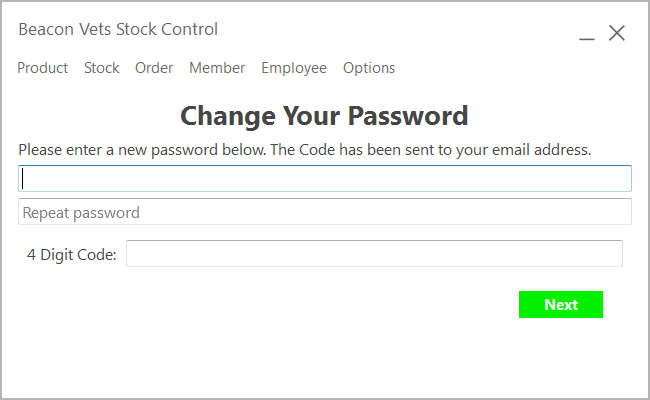
\includegraphics[width=\textwidth]{./interface16.png}
    \caption{Change Password Interface} \label{fig:change-password-interface}
\end{figure}

\subsection{ER Diagram}

Since the Design stage i developed my database and added and removed some tables, that i felt needed to be changed. To see my original ER Diagram from my design, go to page \pageref{fig:ER Diagram}, figure \ref{fig:ER Diagram}. To be able to track the amount of sales made each week and each day for each product so that this data could be plotted onto a graph, i created two new entities.DailyProductSales and WeeklyProductSales, both entities take ProductID as a foreign key and i have also included a seperate table called Settings. The settings tables simple stores the preferences entered by the user and has no relationship with any of the other data. below is my new ER Diagram, i have removed Location and Product location as these entities were not needed.

\begin{figure}[H]
    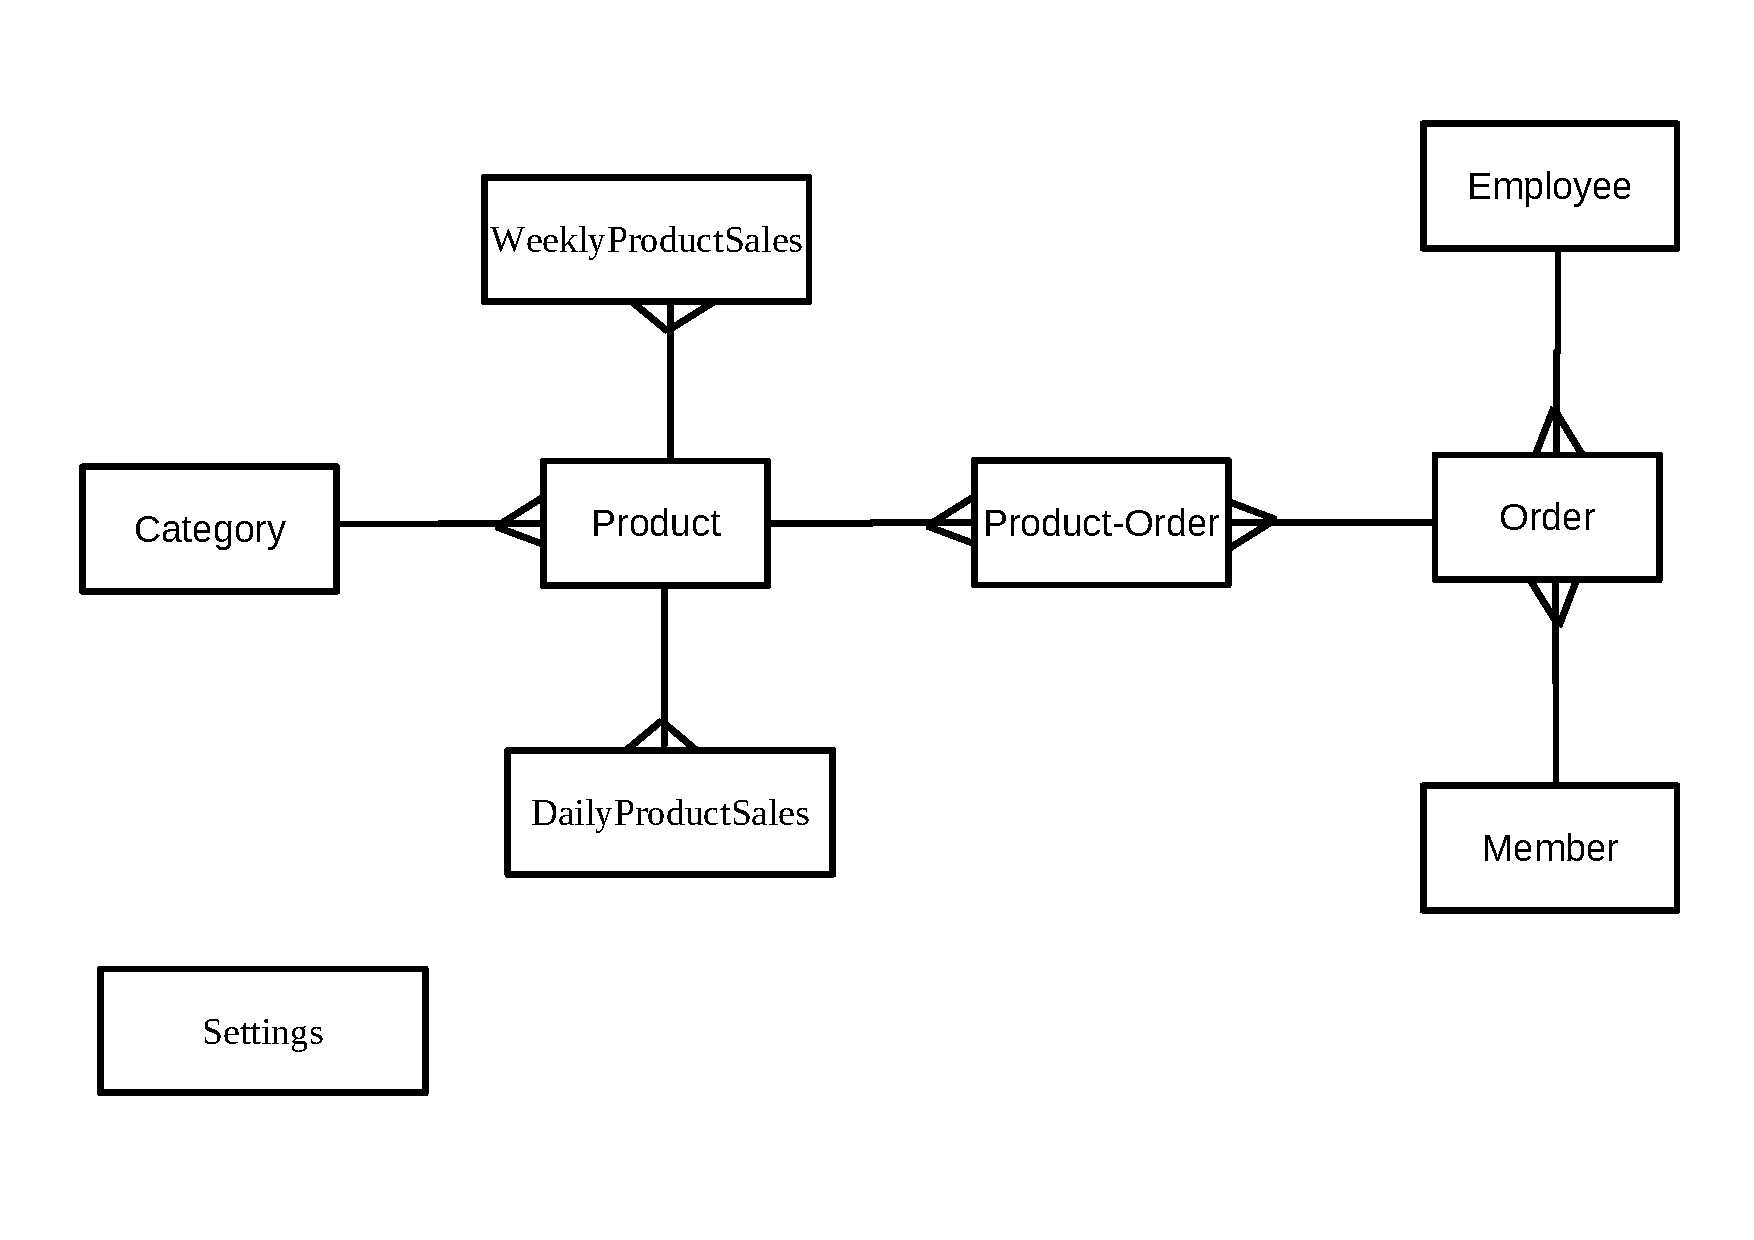
\includegraphics[width=\textwidth]{./ERDiagramMaintenance.pdf}
    \caption{New Entity Relationship Diagram} \label{fig:entity-relationship-maintenance}
\end{figure}

\subsection{Database Table Views}

\begin{figure}[H]
    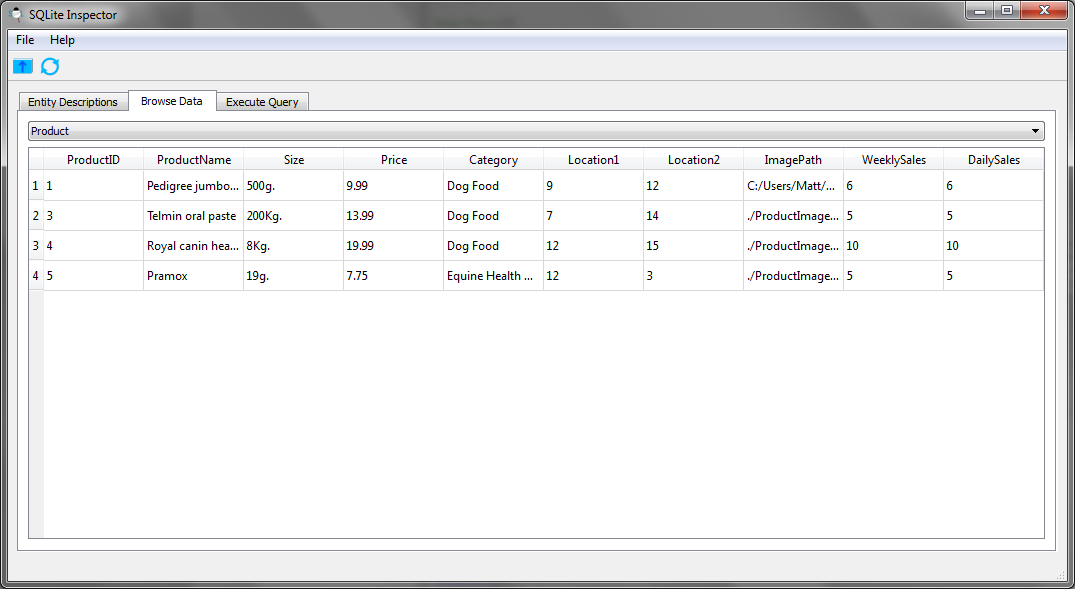
\includegraphics[width=\textwidth]{./TableView1.png}
    \caption{New Entity Relationship Diagram} \label{fig:table-view-1}
\end{figure}

\begin{figure}[H]
    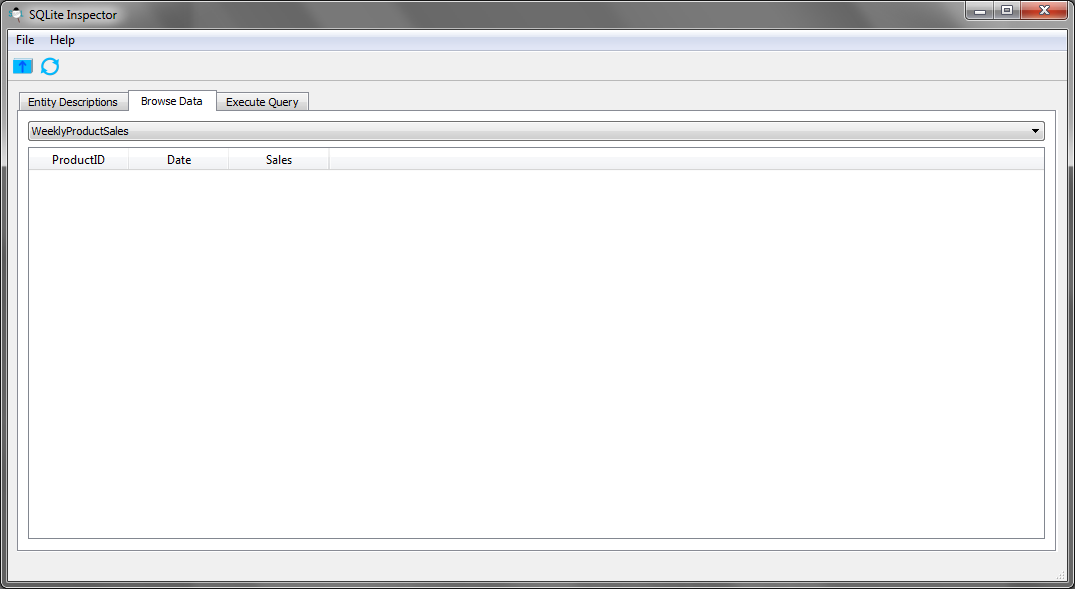
\includegraphics[width=\textwidth]{./TableView2.png}
    \caption{New Entity Relationship Diagram} \label{fig:table-view-2}
\end{figure}

\begin{figure}[H]
    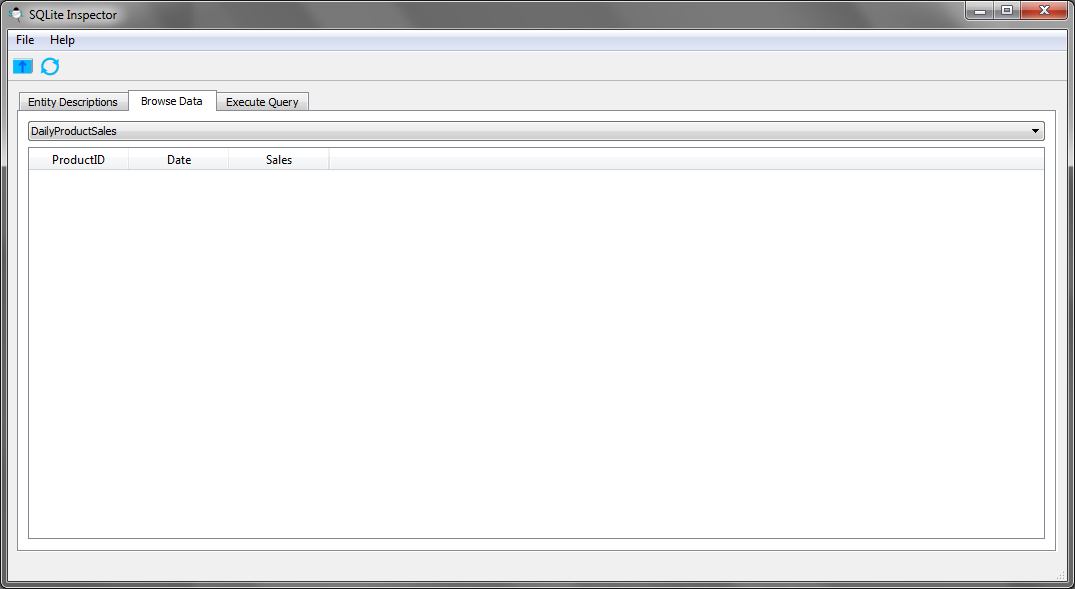
\includegraphics[width=\textwidth]{./TableView3.png}
    \caption{New Entity Relationship Diagram} \label{fig:table-view-3}
\end{figure}

\begin{figure}[H]
    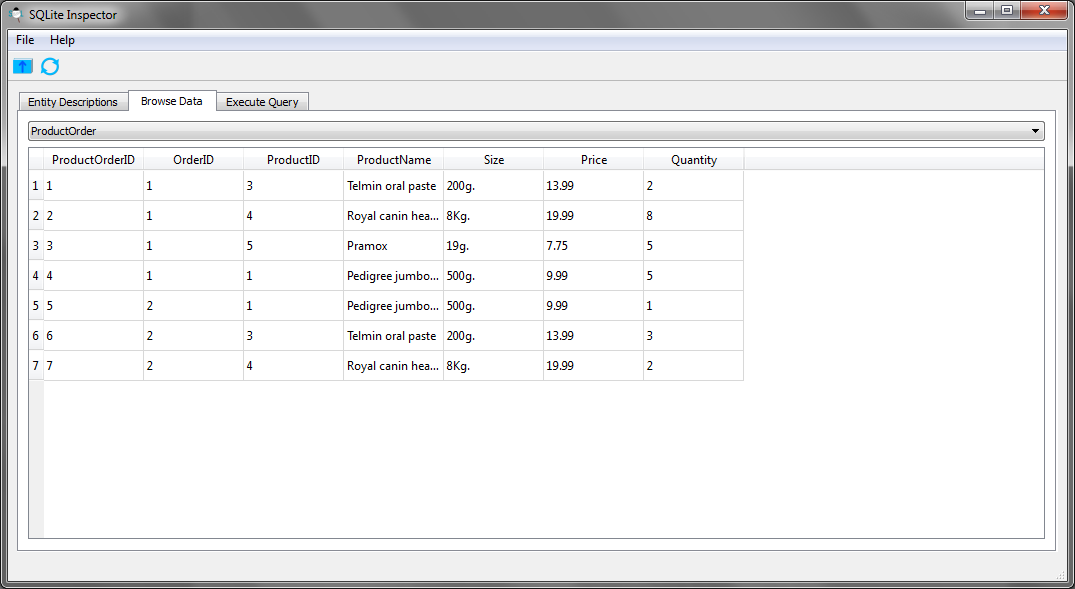
\includegraphics[width=\textwidth]{./TableView4.png}
    \caption{New Entity Relationship Diagram} \label{fig:table-view-4}
\end{figure}

\begin{figure}[H]
    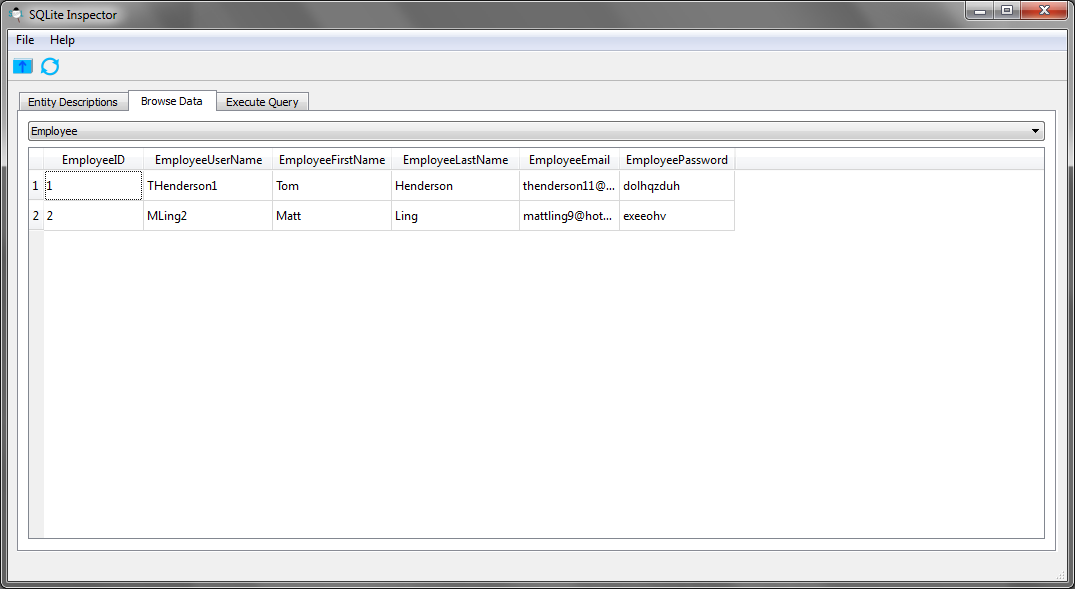
\includegraphics[width=\textwidth]{./TableView5.png}
    \caption{New Entity Relationship Diagram} \label{fig:table-view-5}
\end{figure}

\begin{figure}[H]
    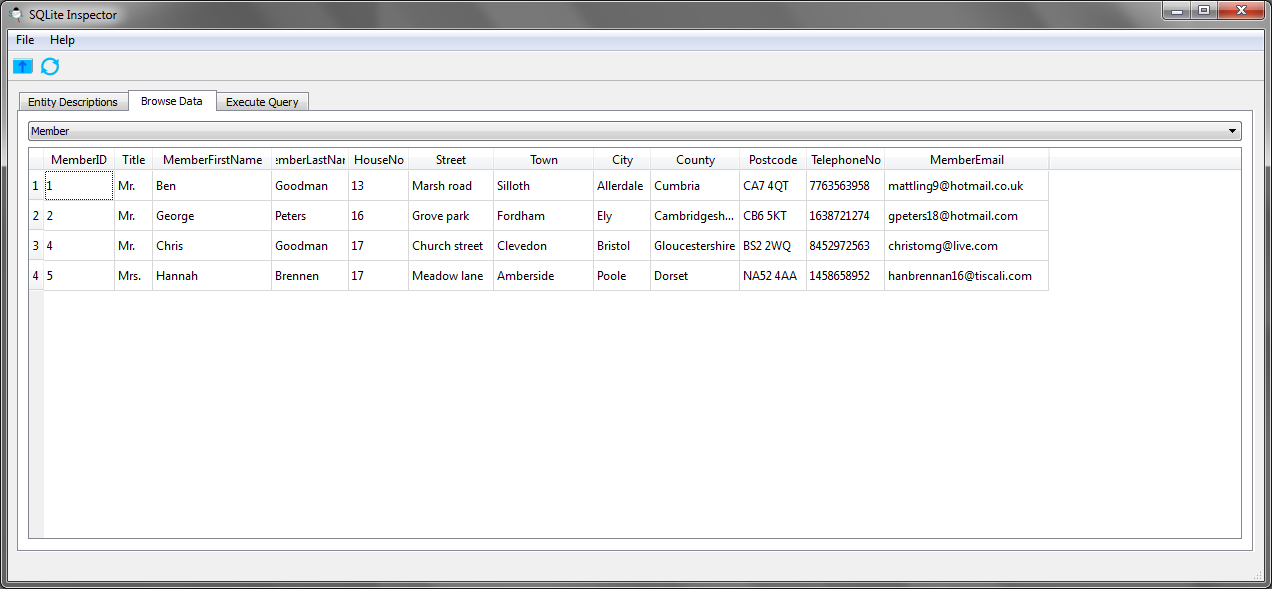
\includegraphics[width=\textwidth]{./TableView6.png}
    \caption{New Entity Relationship Diagram} \label{fig:table-view-6}
\end{figure}

\begin{figure}[H]
    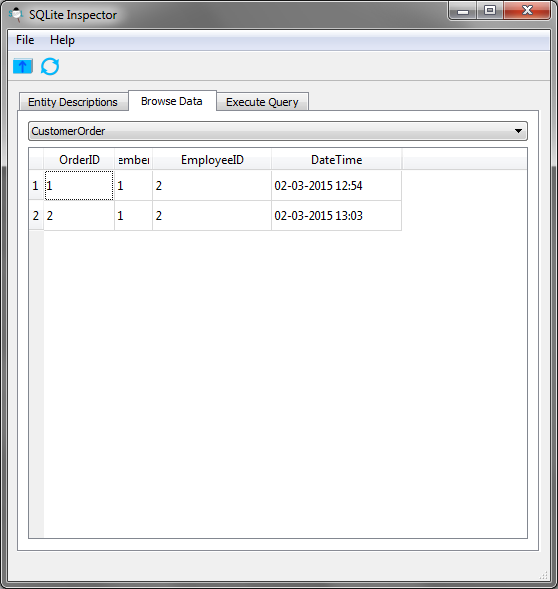
\includegraphics[width=\textwidth]{./TableView7.png}
    \caption{New Entity Relationship Diagram} \label{fig:table-view-7}
\end{figure}

\begin{figure}[H]
    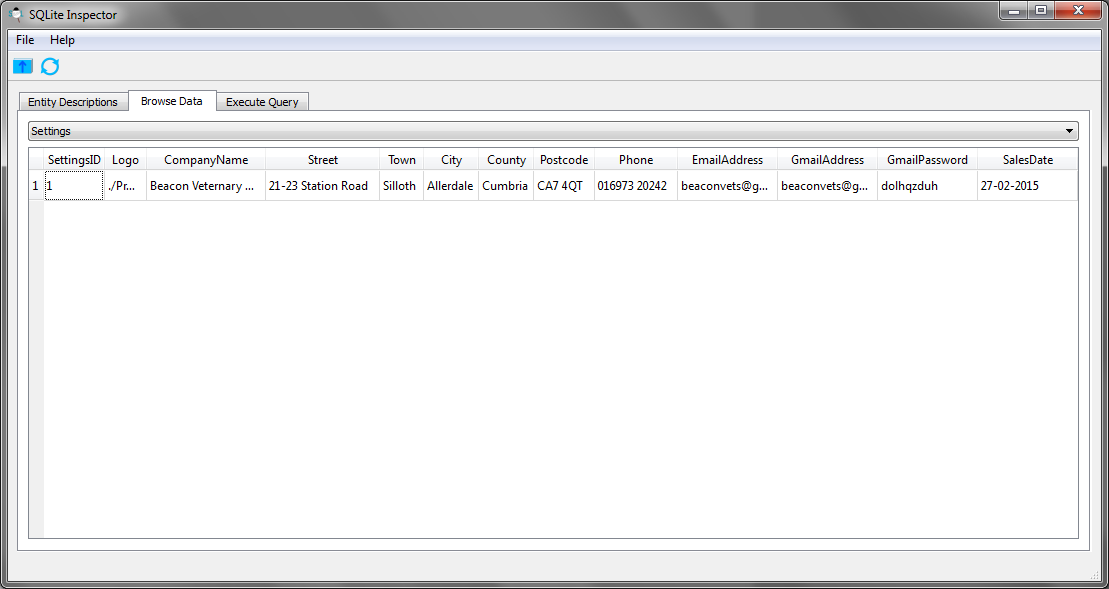
\includegraphics[width=\textwidth]{./TableView8.png}
    \caption{New Entity Relationship Diagram} \label{fig:table-view-8}
\end{figure}


\subsection{Database SQL}

\subsection{SQL Queries}

\section{Testing}

\subsection{Summary of Results}

\subsection{Known Issues}

\section{Code Explanations}

\subsection{Difficult Sections}

\subsection{Self-created Algorithms}

\section{Settings}

When managing the stock of the products, the user gets displayed a graph which shows the sales of the product either by week or by day. This graph was implemented into my system using the matplotlib library. The matplotlib library does not come with the installation in python. The easiest way to install matplotlib is by using PIP, a tool that does come with the python installation that installs the library you want, along with all the dependencies it requires to work. To install pip on Windows, the user can type `` python3 get-pip.py'' into the command prompt. Then to install matplotlib, the user can then type ``pip install matplotlib'' which should start to download and install matplotlib and all of its dependencies. If you do not want to install matplotlib using pip, it can be installed manually, however, you are required to install several other modules manually as well. Other than matplotlib, all of the other modules used in my system come pre-installed with either python, PyQt or SQLite 3.


.

\section{Acknowledgements}

\pagebreak

\section{Code Listing}


\subsection{Main Program}
\pythonfile{./Maintenance/Main.py}
\pagebreak

\subsection{Adding Product}
\pythonfile{./Maintenance/AddingProductClass.py}
\pagebreak


\subsection{Editing Product}
\pythonfile{./Maintenance/EditProductClass.py}
\pagebreak

\subsection{Removing Product}
\pythonfile{./Maintenance/DeleteProductClass.py}
\pagebreak

\subsection{Adding Member}
\pythonfile{./Maintenance/AddingMemberClass.py}
\pagebreak

\subsection{Editing Member}
\pythonfile[firstline=1]{./Maintenance/EditMemberClass.py}
\pagebreak

\subsection{Deleting Member}
\pythonfile[firstline=1]{./Maintenance/DeleteMemberClass.py}
\pagebreak


\subsection{Adding Employee}
\pythonfile[firstline=1]{./Maintenance/AddingEmployeeClass.py}
\pagebreak


\subsection{Editing Employee}
\pythonfile[firstline=1]{./Maintenance/EditEmployeeClass.py}
\pagebreak


\subsection{Deleting Employee}
\pythonfile[firstline=1]{./Maintenance/DeleteEmployeeClass.py}
\pagebreak


\subsection{Log In Screen}
\pythonfile[firstline=1]{./Maintenance/LogInClass.py}
\pagebreak


\subsection{Preferences Interface}
\pythonfile[firstline=1]{./Maintenance/PreferencesClass.py}
\pagebreak


\subsection{Stock Management Interface}
\pythonfile[firstline=1]{./Maintenance/StockManagementClass.py}
\pagebreak


\subsection{SQL Queries}
\pythonfile[firstline=1]{./Maintenance/AddingRemovingData.py}
\pagebreak

\subsection{Changing Password Interface}
\pythonfile[firstline=1]{./Maintenance/ChangePasswordClass.py}
\pagebreak


\subsection{Creating Order Interface}
\pythonfile[firstline=1]{./Maintenance/CreatingOrderClass.py}
\pagebreak


\subsection{Search Window}
\pythonfile[firstline=1]{./Maintenance/FindingPopUpClass.py}
\pagebreak


\subsection{Order Interface}
\pythonfile[firstline=1]{./Maintenance/CreatingOrderClass.py}
\pagebreak


\subsection{Message with a single Ok button}
\pythonfile[firstline=1]{./Maintenance/ErrorMessageClass.py}
\pagebreak


\subsection{Message with Yes and No buttons}
\pythonfile[firstline=1]{./Maintenance/PopUpMenuClass.py}
\pagebreak


\subsection{Search Window}
\pythonfile[firstline=1]{./Maintenance/FindingPopUpClass.py}
\pagebreak


\subsection{Password Reset Interface}
\pythonfile[firstline=1]{./Maintenance/PasswordResetClass.py}
\pagebreak


\subsection{Custom Window Frame}
\pythonfile[firstline=1]{./Maintenance/CustomToolbarClass.py}
\pagebreak


\subsection{SQL Connections}
\pythonfile[firstline=1]{./Maintenance/SQLConnection.py}
\pagebreak


\subsection{Clickable QLabel}
\pythonfile[firstline=1]{./Maintenance/ExtendedQLabel.py}
\pagebreak


\subsection{Creating the Tables in the database.}
\pythonfile[firstline=1]{./Maintenance/CreatingTable.py}
\pagebreak


\subsection{Style sheet for Main Window}
\pythonfile[firstline=1]{./Maintenance/StyleSheet.py}
\pagebreak
